% !TeX spellcheck = en_US
\documentclass[]{article}


%opening
\title{Current Topics in Multimedia Communication: Server, Cluster, and Cloud Computing}

\author{Giovanni Liva}

\usepackage[T1]{fontenc}
\usepackage[english]{babel}
%\usepackage[utf8]{inputenc}
\usepackage[latin1]{inputenc}
\usepackage{graphicx}
\usepackage{amsmath}
\usepackage{mathtools}
\usepackage{amsfonts}
\usepackage[final]{pdfpages}
\usepackage{subcaption}
\usepackage{geometry}
\usepackage{hyperref}
\hypersetup{
	colorlinks   = true,    % Colours links instead of ugly boxes
	urlcolor     = blue,    % Colour for external hyperlinks
	linkcolor    = blue,    % Colour of internal links
	citecolor    = red      % Colour of citations
}
\newcommand{\norm}[1]{\left\lVert#1\right\rVert}

\usepackage{wrapfig}
\usepackage{lscape}
\usepackage{rotating}
\usepackage{epstopdf}
\usepackage{float}
\usepackage{listings}


\lstdefinestyle{customc}{
    belowcaptionskip=1\baselineskip,
    breaklines=true,
    frame=L,
    xleftmargin=\parindent,
    language=C++,
    showstringspaces=false,
    basicstyle=\footnotesize\ttfamily,
    keywordstyle=\bfseries\color{green!40!black},
    commentstyle=\itshape\color{purple!40!black},
    identifierstyle=\color{blue},
    stringstyle=\color{orange},
}

\begin{document}
\captionsetup[figure]{font=small,skip=0pt}
\maketitle


\section{Introduction}
All the code was written in C/C++ using only the standard libraries. 
The compiler used is \textit{clang} version \texttt{703.0.31} on OSX  \texttt{10.10.4}.
In order to compile the project, the only operation needed is to run the \texttt{make} command in the directory that contains the \texttt{Makefile} file.
The arguments accepted by the program are the following:
\begin{itemize}
    \item -row [n] : set the number of rows to \textit{n} for matrices A, B and C.
    \item -col [n] : set the number of columns to \textit{n} for matrices A, B and C.
    \item -fill [n] : set the filling percentage to \textit{n} for matrices A and B.
    \item -t [n] : set the number of thread to use to \textit{n}, the default value is 1.
    \item -d : allows the debug mode. This modality prints in the standard output some debug info and print the matrices in csv files.
    \item -s [n] : set the strategy to use to compute the addiction of the matrices to \textit{n}, the default value is 0. The possible values are: \textit{0, 1, 2, 3}. Further details about the strategies are given in Section \ref{strategy}.
    \item -f [filename] : store data about the computation in the specified file in csv format. If the file already exists, the data will be appended to the current one. This parameter is used to store the data used in Section \ref{evaluation}.
\end{itemize}
The first two parameters are mandatory.
All the tests were done on the following hardware:
\begin{itemize}
    \item processor: 2,5 GHz Intel Core i7-4870HQ \footnote{\url{http://ark.intel.com/products/83504/Intel-Core-i7-4870HQ-Processor-6M-Cache-up-to-3_70-GHz}}
    \item number of cores: 4
    \item number of threads: 8
    \item ram: 16 GB
\end{itemize}


\section{Implementation}
The project was created in two C/C++ files with their own headers: \texttt{Main.cpp} and \texttt{YSMF.cpp}.
In the following section we will discuss the relevant parts of  code of these two files.
As a requirement for this project, the \texttt{pthread} library is used instead of the \texttt{std::thread} library.
\paragraph{YSFM.cpp}
The implementation of the YSMF is coded as C++ class. The whole code is straightforward since it implements some getters to the three vectors that store the information in the Yale Sparse Matrix Format.
The filling strategy uses a random distribution to decide where to store a integer that is a randomly generated in the interval $[1,9]$. The random distribution tends to store more data in the last rows of the matrix.
The interesting part of code of this class are following two methods.

\label{addElement}
\begin{lstlisting}[style=customc]
void YSMF::addElement(int elm, int row, int col) {
    if(elm == 0) return;
    A.push_back(elm);
    JA.push_back(col);
    for(int i = row+1; i <= _nRows; i++){
        IA[i] += 1;
    }
    NNZ++;
}
\end{lstlisting}
\label{addElementThread}
\begin{lstlisting}[style=customc]
void YSMF::addElementThread(int elm, int row, int col, int nElmSkip){
    if(elm == 0) return;
    //create memory for new elements
    if (nElmSkip >= A.size()) {
        A.resize(nElmSkip+1);
    }
    if (nElmSkip >= JA.size()) {
        JA.resize(nElmSkip+1);
    }
    A.insert(A.begin() + nElmSkip, elm);
    JA.insert(JA.begin() + nElmSkip, col);
    for(int i = row+1; i <= _nRows; i++){
        IA[i] += 1;
    }
    NNZ++;
}
\end{lstlisting}
The \texttt{YSMF::addElement} method insert an element in the position specified in the parameters.
Since the \texttt{YSMF} uses an encoding left to right, top to bottom of the elements, we have to implement a different method if we want to allow an insertion that does not respect that order.
This method is mandatory since we would like to compute sum of matrices in parallel.
For this reason the \texttt{YSMF::addElementThread} method has a parameter that specifies where in $A$ and $JA$ we will insert the new element.

\newpage
\label{Main}
\paragraph{Main.cpp}
This file, as the name suggests, implements the main function and the logic to parse the parameters and to spawn the threads.
After parsing the input parameters, it creates the data to pass to each thread. We refer to this phase of creation of data as \textit{init phase of threads}. After the \textit{init phase} it creates the threads using the specified strategy and then wait until all of them end their computation.




\label{strategy}
\subsection{Strategies}
We look at the Yale Sparse Matrix Format and we decided that the computation of the addiction of the two matrices can be performed in different ways. 
\textit{Strategy 0} and \textit{Strategy 1} use a na\"ive approach.
They go through all the matrices position and check if there is an element stored in that particular position.
\textit{Strategy 2} instead pre-process the two matrices in order to go through only the elements stored.
Further, if we divide the workload of  threads in rows of C to compute, we can avoid to use synchronization method because there are only concurrent reads. \textit{Strategy 1} and \textit{3} implement this approach using a small local matrix to store the results. When all the threads join, all the local matrices are merged to compute the correct $C$ matrix.
In each strategy, we give an $id$ to each thread. This $id$ is unique and in the range $[0, \#thread-1]$, where $\#thread$ is the number specified as parameter.

\paragraph{Init Phase Strategy 0 and 1}
The creation of data for these two strategy is simple, we just have to specify the range of rows where the thread has to compute the sum and initialize the local matrix where to store the results for \textit{Strategy 1}.
\begin{lstlisting}[style=customc]
int batch_size = n_row / n_thread;
for(int i = 0; i < n_thread; i++){
    _data[i].id = i;
    _data[i].start = batch_size * i;
    _data[i].end = (i == n_thread-1) ? n_row :  _data[i].start + batch_size;
    _data[i].c = new YSMF(_data[i].end-_data[i].start, n_col);
}
\end{lstlisting}

\paragraph{Init Phase Strategy 2 and 3}
These two strategies uses the same init phase of the previous ones plus some more work.
We store the elements of $A$ and $B$ in two \texttt{std::map} data structure. The current pre-process of the data allows the \textit{Strategy 2} and \textit{3} to go through only the elements of $A$ and $B$ and skip the empty zones of the matrices.
The workload of threads here is divided in the same manner of the previous strategies.
\begin{lstlisting}[style=customc]
std::vector<std::pair<int, int>> coordinateA = a->getElmCoordinate();
std::vector<int> *aA = a->getA();
for(int i = 0; i < coordinateA.size(); i++){
    mapA[coordinateA[i].first][coordinateA[i].second] = aA->at(i);
}
std::vector<std::pair<int, int>> coordinate = b->getElmCoordinate();
std::vector<int> *bA = b->getA();
for(int i = 0; i < coordinate.size(); i++){
    mapB[coordinate[i].first][coordinate[i].second] = bA->at(i);
}
\end{lstlisting}



\label{strategy:0}
\paragraph{Strategy 0}
The code of the strategy is the following:
\begin{lstlisting}[style=customc]
struct threadData *data = (struct threadData *)arg;
int maxColB = b->getCols();
int sum ;
int startLine = data->start;
int endLine = data->end;
int NNZ = 0;
//work only on out batch size
for(int i = startLine; i < endLine; i++){
    for(int j = 0; j < maxColB; j++){
        sum = a->getElement(i,j) + b->getElement(i, j);
        if(sum > 0) {
            //check where store the data
            NNZ = 0;
            pthread_mutex_lock(&lock);
            for(int z = 0; z <= data->id; z++){
                NNZ += nElmWrite[z];
            }
            //write down the result
            c->addElementThread(sum, i, j, NNZ);
            nElmWrite[data->id]++;
            pthread_mutex_unlock(&lock);
        }
    
    }
}
\end{lstlisting}
It goes through all the rows and columns of $A$ and $B$ and compute the sum.
The vector $nElmWrite$ is a global vector share between each thread that stores the information about how many elements that particular thread has compute. This is mandatory because we have to track how many element the threads with $id$ lower than the $id$ of the current one have written. This assumption of correctness of the algorithm holds since we give horizontal slice of the matrix C to compute to each thread and the slice have the same order of the $ids$ of the threads. This allows the algorithm to fulfill the requirement to write elements in left to right, top to bottom order.

\newpage
\label{strategy:1}
\paragraph{Strategy 1}
The code of \textit{Strategy 1} is the following:
\begin{lstlisting}[style=customc]
struct threadData *data = (struct threadData *)arg;
int maxColB = b->getCols();
int sum ;
int startLine = data->start;
int endLine = data->end;
//work only on our batch size
for(int i = startLine; i < endLine; i++){
    for(int j = 0; j < maxColB; j++){
        sum = a->getElement(i,j) + b->getElement(i, j);
        if(sum > 0) {
            data->c->addElement(sum,i - startLine,j);
        }
    }
}
\end{lstlisting}
The code is similar to the one of the previous strategy. The only difference is that now we do not have any protect regions and we write locally the result of the sum.
This strategy has to perform some work for merging the results after the join operation.
\begin{lstlisting}[style=customc]
int sumElms = 0;
int pos = 0;
for(int i = 0; i < n_thread; i++){
    //merge results
    std::vector<int> *tA = _data[i].c->getA();
    std::vector<int> *tIA = _data[i].c->getIA();
    std::vector<int> *tJA = _data[i].c->getJA();
    cA->reserve(cA->size() + tA->size());
    cA->insert(cA->end(), tA->begin(), tA->end());
    cJA->reserve(cJA->size() + tJA->size());
    cJA->insert(cJA->end(), tJA->begin(), tJA->end());
    //full fill spaces
    int max = _data[i].c->getRows();
    for(int k = 1; k <= max; k++){
        cIA->at(++pos) = tIA->at(k) + sumElms;
    }
    sumElms += tIA->at(max);
}
\end{lstlisting}
Vector $A$ and $JA$ are computed append the ones of each thread. Regarding $IA$ instead we have also to remember the number of element that each thread compute.
\newpage
\label{strategy:2}
\paragraph{Strategy 2}
The code of \textit{Strategy 2} is the following:
\begin{lstlisting}[style=customc]
struct threadData *data = (struct threadData *)arg;
int start = data->start;
int end = data->end;
int maxColB = b->getCols();
int row,col,sum;
for (row = start; row < end; row++) {
    if(mapA.count(row) < 1 && mapB.count(row) < 1){
        continue;
    }
    //for each col of B
    for(col = 0; col < maxColB; col++){
        sum = 0;
        if(mapA.count(row) > 0 && mapA[row].count(col) > 0){
            sum += mapA[row][col];
        }
        if(mapB.count(row) > 0 && mapB[row].count(col) > 0){
            sum += mapB[row][col];
        }
        if(sum > 0){
            int z = 0;
            int NNZ = 0;
            pthread_mutex_lock(&lock);
            for(; z <= data->id; z++){
                NNZ += nElmWrite[z];
            }
            //write down the result
            c->addElementThread(sum, row, col, NNZ);
            nElmWrite[data->id]++;
            pthread_mutex_unlock(&lock);
        }
    }
}
\end{lstlisting}
It is similar to the first strategy, except for the using of the map.
The motivation for introducing such strategy is given looking through the code of \texttt{YSMF::getElement}.
\begin{lstlisting}[style=customc]
int YSMF::getElement(int i, int j){
    int d = IA[i+1] - IA[i];
    if(d > 0){
        std::pair<std::vector<int>, std::vector<int>> row = getRow(i);
        for(int k = 0; k < row.first.size(); k++){
            if(j == row.second[k])
            return row.first[k];
        }
    }
    return 0;
}
\end{lstlisting}
Since in the previous strategies call it many times it makes the code go through the for many times and for each row always looking just one more element of the column.
To avoid this, we decided to pre-process the matrices in order to do the work only once.

\newpage
\label{strategy:3}
\paragraph{Strategy 3}
The code of \textit{Strategy 3} is the following:
\begin{lstlisting}[style=customc]
struct threadData *data = (struct threadData *)arg;
int start = data->start;
int end = data->end;
int maxColB = b->getCols();
int row,col,sum;
for (row = start; row < end; row++) {
    if(mapA.count(row) < 1 && mapB.count(row) < 1){
        continue;
    }
    //for each col of B
    for(col = 0; col < maxColB; col++){
        sum = 0;
        if(mapA.count(row) > 0 && mapA[row].count(col) > 0){
            sum += mapA[row][col];
        }
        if(mapB.count(row) > 0 && mapB[row].count(col) > 0){
            sum += mapB[row][col];
        }
        if(sum > 0){
            data->c->addElement(sum,row - start,col);
        }
    }
}
\end{lstlisting}
It combines all the purpose of \textit{Strategy 2} with the idea of using a local matrix to avoid synchronization of \textit{Strategy 1}.

\label{evaluation}
\section{Evaluation}
All the data is computed running the  \texttt{./evaluation.sh} script.
That script is divided in three sections and each one computes only square matrices.
In the first part we execute the program multiple time varying the number of rows and columns using only one thread.
In the second section the size of the matrix is fixed to $3000\times 3000$, but we change the number of threads to use, from $2$ to $80$ with a step of $2$.
In the latter part, we execute strategy number one and three in the same settings of the second evaluation but with a matrix size of $15000\times 15000$. 
The last evaluation was necessary to completely check how much time with \textit{Strategy 3} the \textit{init phase} of the data takes with a matrix that requires some time to be process.
\newpage
\paragraph{Single Thread}
Figure \ref{fig:all_single} shows the time necessary to compute the addiction of the matrices for all the four strategies. 
The graph confirms out expectation, pre-process the data with \textit{Strategy 2} and \textit{3} reduces the time to compute the addiction.
Moreover, it confirms that using locking strategies or not, does not impact the result since there is not any race to a common resource.
\begin{figure}[H]
	\centering
	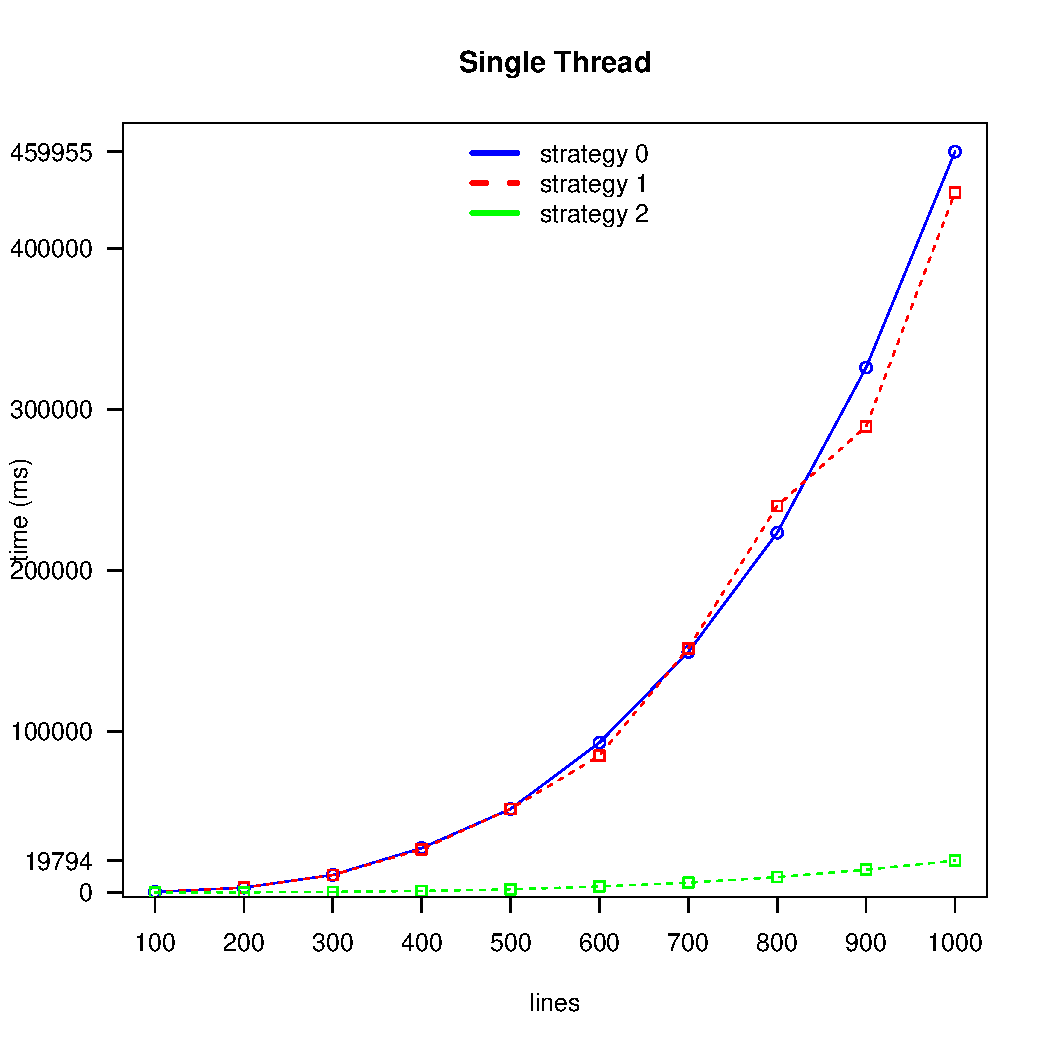
\includegraphics[width=1\textwidth]{img/all_single.pdf}
	\caption
	{Time to compute the addiction with a single thread.}
	\label{fig:all_single}
\end{figure}

\newpage
\paragraph{Multiple Thread}
Figure \ref{fig:all_multiple} presents some behaviors that we do not await. All the strategies compute a matrix $3000\times 3000$ with different number of threads. If we compare the result for each strategy in a singular thread, \textit{Strategy 0} and \textit{2} perform always worst with multi-thread. We do not foresee such behavior and we dig into the code to find some bugs that can cause the reduction of performance, but we did not manage to discover anything. Nevertheless, the Figure shows a confirmed that increasing too much the number of threads we decrease the performances. This attitude does not appear in \textit{Strategy 1} and \textit{3} because the matrix to compute is too small.
\begin{figure}[H]
	\centering
	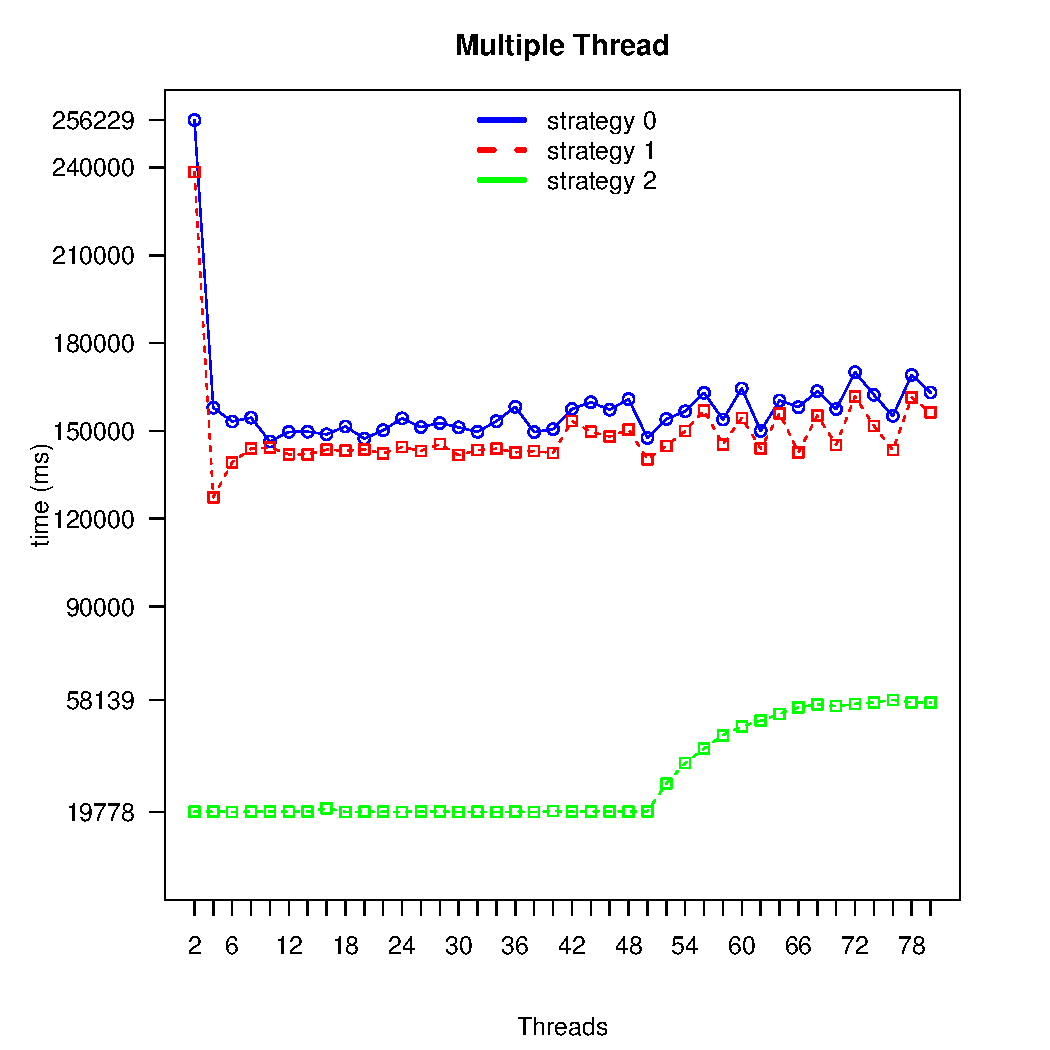
\includegraphics[width=1\textwidth]{img/all_multiple.pdf}
	\caption
	{Time required to compute a matrix $3000\times 3000$ with different number of threads.}
	\label{fig:all_multiple}
\end{figure}

\newpage
\paragraph{Speed Up}
We compute the P value comparing the results in multiple-threading evaluation with the equivalent in single-thread settings in terms of matrix size.  Figure \ref{fig:speed_up} presents the values. 
As we expected, for \textit{Strategy 1} and \textit{3}, the P value is greater than $1$ and increasing the number of threads to use, it slowly decreases.
Instead, \textit{Strategy 0} and \textit{2} have a stable value around $0.018$. This means that the two strategies are not suitable at all for multi-thread execution.
\begin{figure}[H]
    \centering
    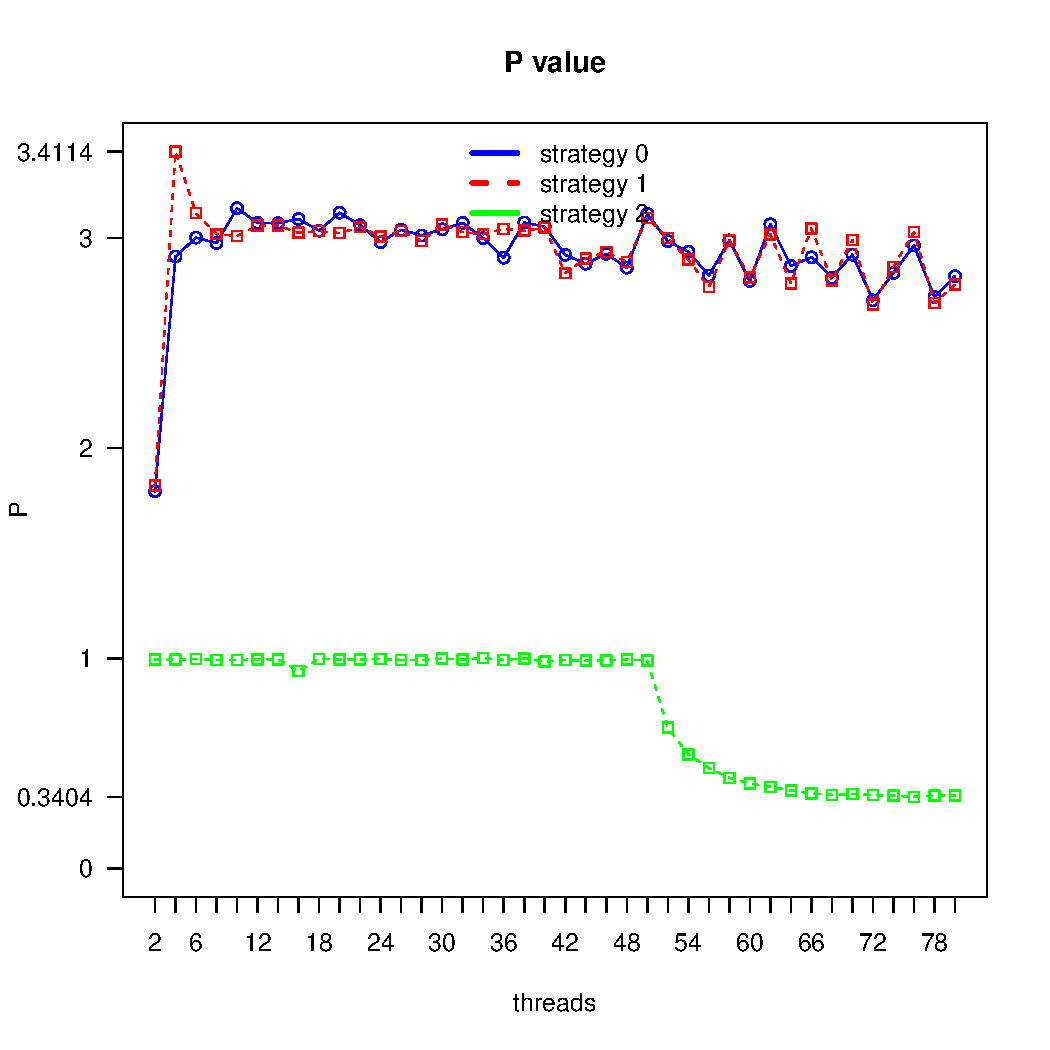
\includegraphics[width=1\textwidth]{img/speedup.pdf}
    \caption
    {P value for each number of thread used.}
    \label{fig:speed_up}
\end{figure}

\newpage
\paragraph{Overhead of Init Phase}
Figure \ref{fig:init} displays how much time \textit{Strategy 2} and \textit{3} spend on pre-process the data in the map structure. \textit{Strategy 2} spent in average roughly $7.5\%$ of its time on the init phase for singular thread and almost $0$ in multi-thread. This trend is confirmed looking to the graphs for its execution time in singular and multi thread. In the singular thread, \textit{Strategy 2} has a good performance that decrease rapidly in the multi-thread experiment.

Regarding \textit{Strategy 3}, it uses more than $70\%$ on preparing the data in the multi-thread setting. This high value is not surprising because the size of the matrix is too small for \textit{Strategy 3} to compute. Figure \ref{fig:str_3_init} shows the time spent on preparing the data for a matrix of $15000$.
Also in this setting the time spent on the init phase takes considerably amount of time, $50\%$, but shows that preparing the data for an efficient process of it improve the performance.

\begin{figure}[H]
    \hspace{-1.7cm}
    \begin{subfigure}{.6\textwidth}
        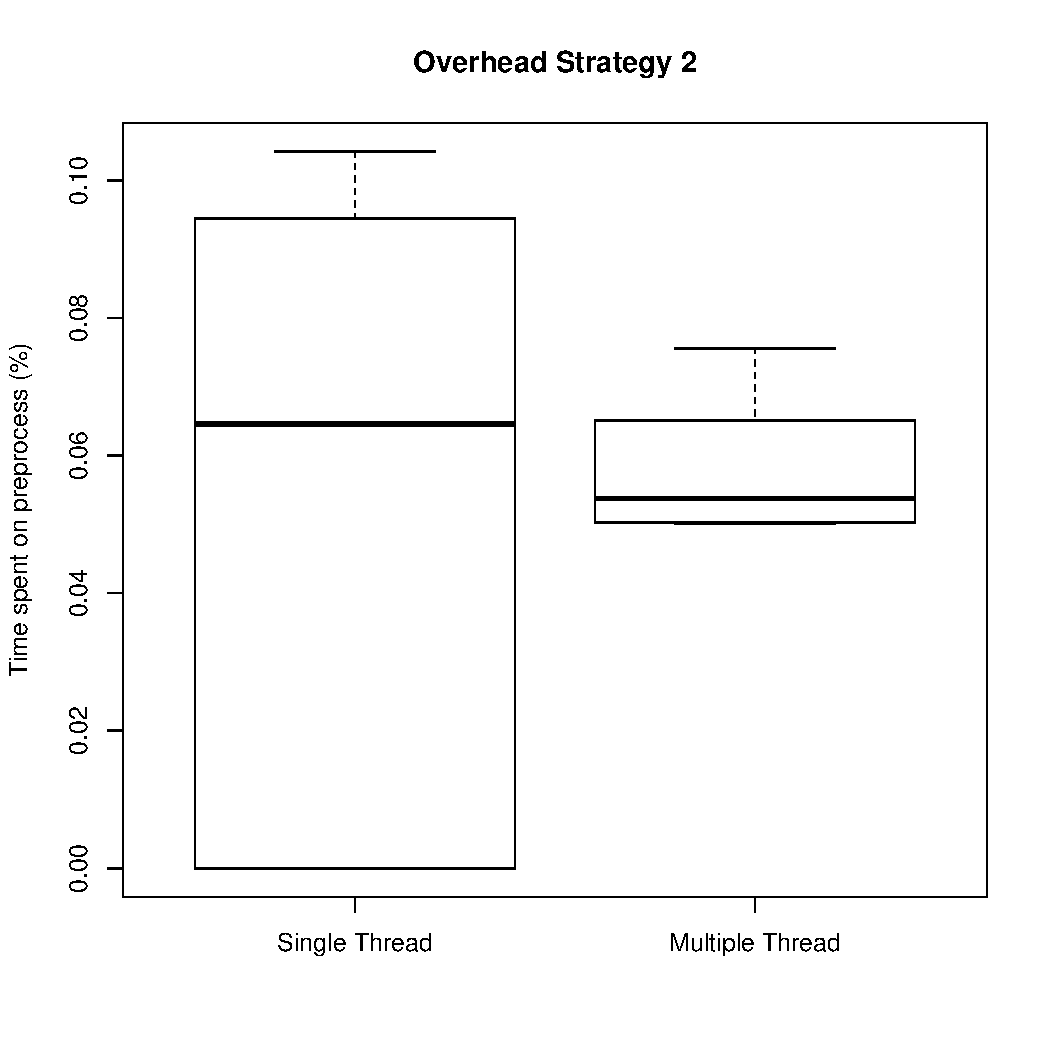
\includegraphics[width=1\textwidth]{img/init_phase.pdf}
        \caption
        {Time spent of pre-process the data.}
        \label{fig:init}
    \end{subfigure}%
    \begin{subfigure}{.6\textwidth}
        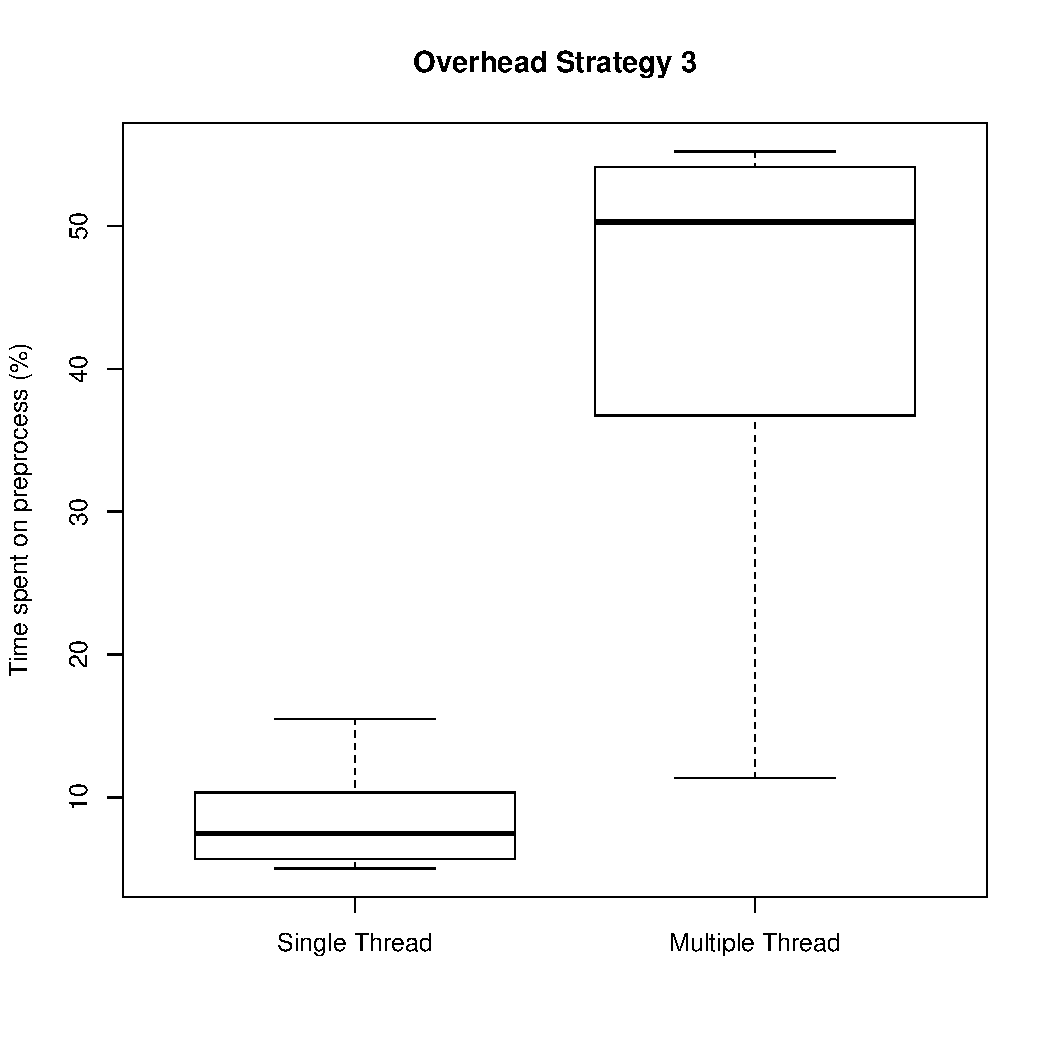
\includegraphics[width=1\textwidth]{img/init_phase_strategy_3.pdf}
        \caption
        {Time spent of pre-process the data with bigger matrix.}
        \label{fig:str_3_init}
    \end{subfigure}%
\end{figure}

\newpage
\newgeometry{bottom=3cm}
\paragraph{Blow the Memory Up}
In order to check the size limit that our hardware can handle we manually run the program increasing the value of cols and rows in the parameters with the fill parameter set to $5\%$.
The maximum value achieved is: $rows=100000, cols=1000000$. That means the program creates two matrices of $100000\times 1000000$ with $5000000000$ non zero elements. The total memory used is presented in Figure \ref{fig:memory_blowed_up}.
If we had to store the two matrices as two dimensional array, it requires $1.6\ TB$ of memory.

\begin{figure}[H]
	\centering
	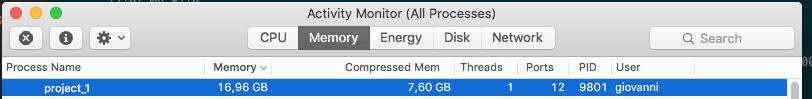
\includegraphics[width=1.15\textwidth]{img/memory_used.png}
	\caption
	{RAM Used to compute two $100000\times1000000$ matrices}
	\label{fig:memory_blowed_up}
\end{figure}

\paragraph{Comparison of Best Strategies}
Since in Figure \ref{fig:all_multiple} is not possible to completely check the performance of \textit{Strategy 1} and \textit{3}, we run these two strategies with a bigger matrix. Figure \ref{fig:strategy_1_3} displays the expected fact of increasing the number of thread after a threshold, it decreases the performance.
\begin{figure}[H]
    \centering
    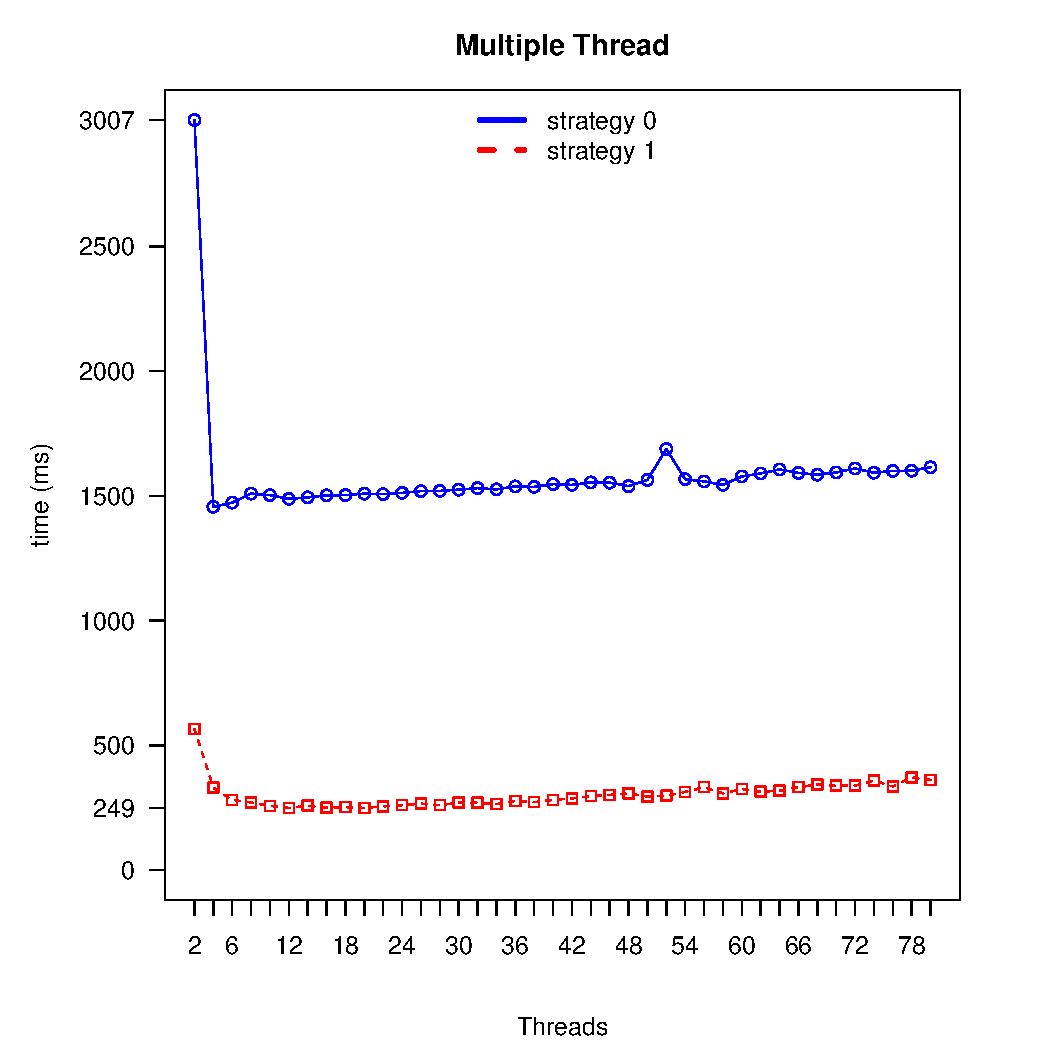
\includegraphics[width=0.8\textwidth]{img/strategy_1_3.pdf}
    \caption
    {Time to compute addiction of $15000\times 15000$ size matrices.}
    \label{fig:strategy_1_3}
\end{figure}


\end{document}
